%!TeX root=../pridetop.tex
\chapter[Chapter \thechapter]{}

\begin{figure}[t!]
\centering
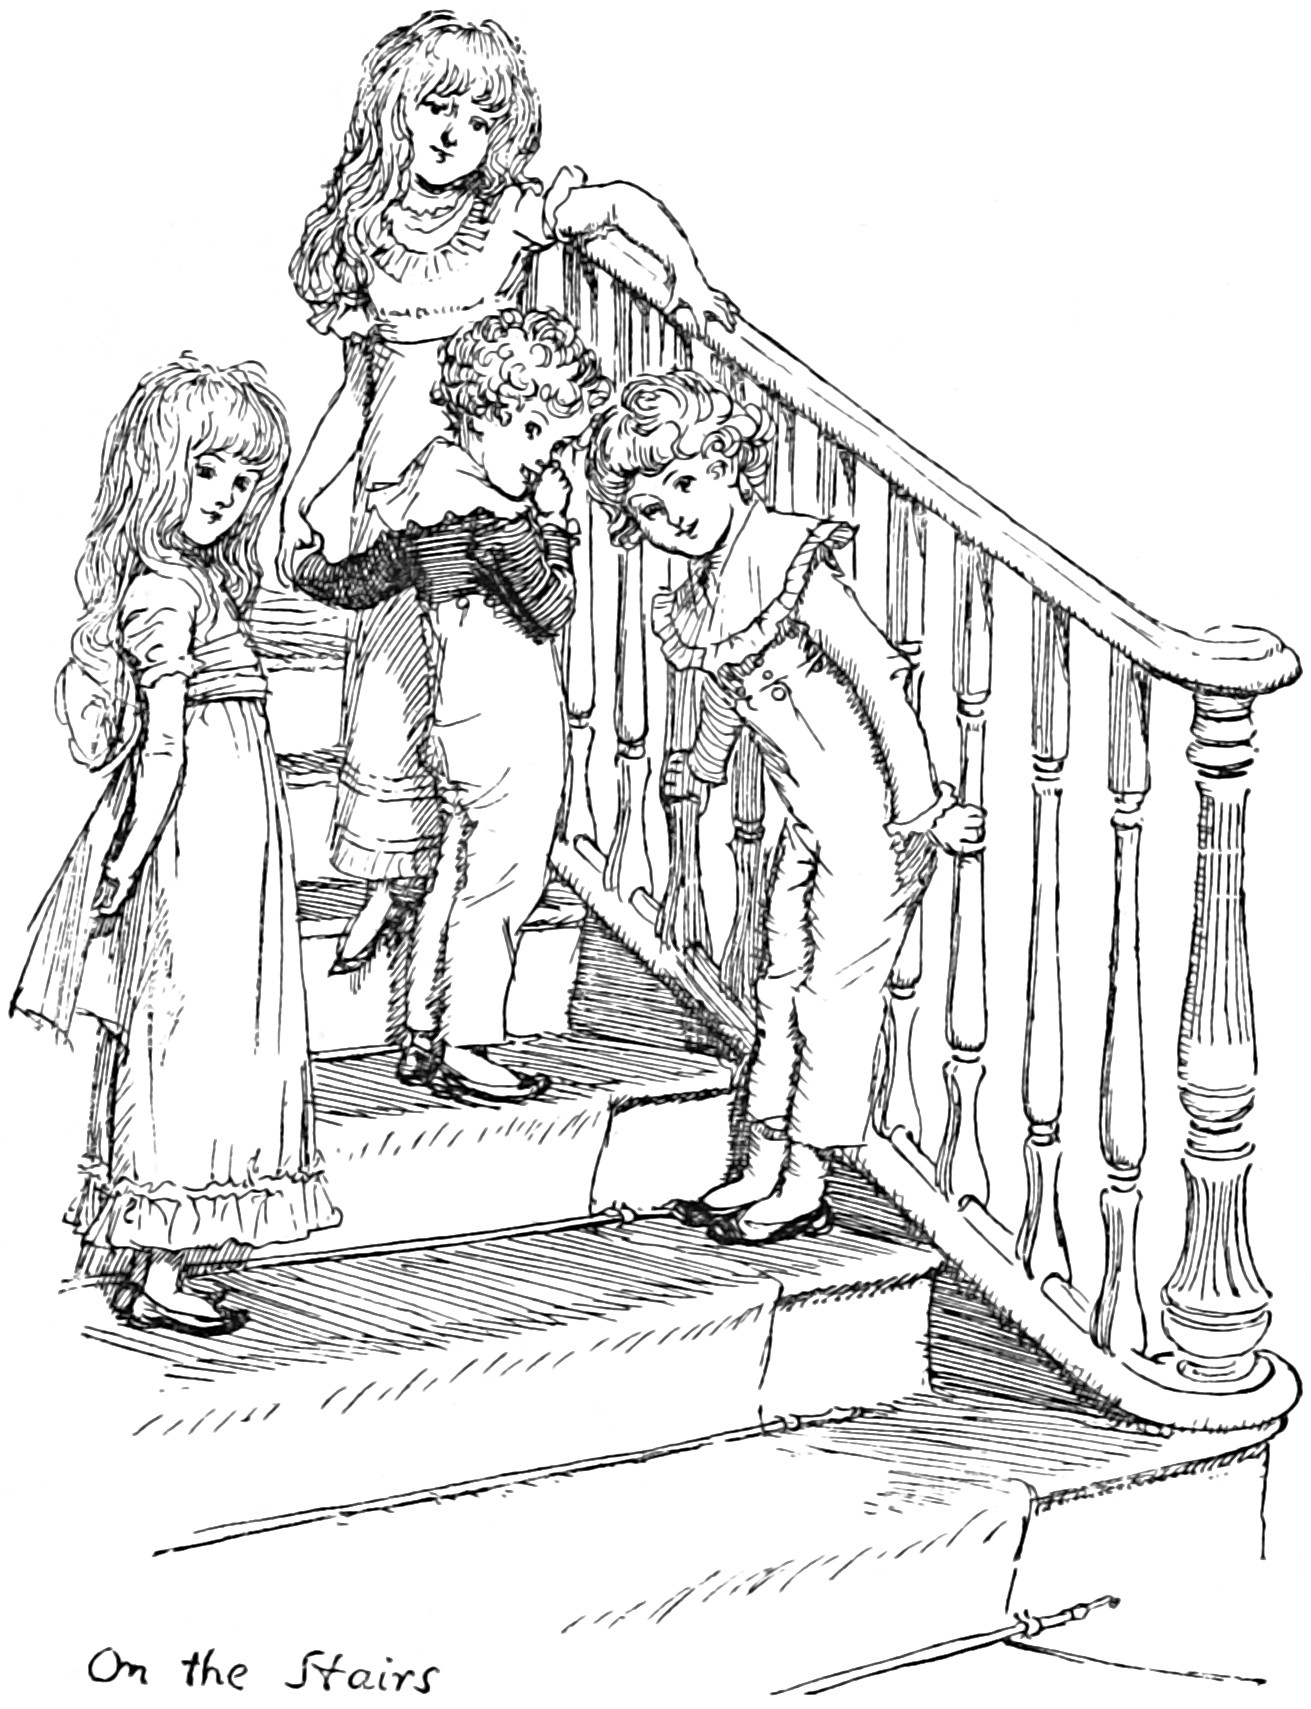
\includegraphics[width=.75\linewidth]{27top}
\captionlistentry{On the stairs}
\end{figure}


\lettrine[lines=6,image=true]{initials/chap27w}{ith}  no greater events than these in the Longbourn family, and otherwise diversified by little beyond the walks to Meryton, sometimes dirty and sometimes cold, did January and February pass away. March was to take Elizabeth to Hunsford. She had not at first thought very seriously of going thither; but Charlotte, she soon found, was depending on the plan, and she gradually learned to consider it herself with greater pleasure as well as greater certainty. Absence had increased her desire of seeing Charlotte again, and weak\-ened her disgust of Mr Collins. There was novelty in the scheme; and as, with such a mother and such uncompanionable sisters, home could not be faultless, a little change was not unwelcome for its own sake. The journey would, moreover, give her a peep at Jane; and, in short, as the time drew near, she would have been very sorry for any delay. Everything, however, went on smoothly, and was finally settled according to Charlotte's first sketch. She was to accompany Sir William and his second daughter. The improvement of spending a night in London was added in time, and the plan became as perfect as plan could be.

The only pain was in leaving her father, who would certainly miss her, and who, when it came to the point, so little liked her going, that he told her to write to him, and almost promised to answer her letter.

The farewell between herself and Mr Wickham was perfectly friendly; on his side even more. His present pursuit could not make him forget that Elizabeth had been the first to excite and to deserve his attention, the first to listen and to pity, the first to be admired; and in his manner of bidding her adieu, wishing her every enjoyment, reminding her of what she was to expect in Lady Catherine de Bourgh, and trusting their opinion of her—their opinion of everybody—would always coincide, there was a solicitude, an interest, which she felt must ever attach her to him with a most sincere regard; and she parted from him convinced, that, whether married or single, he must always be her model of the amiable and pleasing.

Her fellow-travellers the next day were not of a kind to make her think him less agreeable. Sir William Lucas, and his daughter Maria, a good-humoured girl, but as empty-headed as himself, had nothing to say that could be worth hearing, and were listened to with about as much delight as the rattle of the chaise. Elizabeth loved absurdities, but she had known Sir William's too long. He could tell her nothing new of the wonders of his presentation and knighthood; and his civilities were worn out, like his information.

It was a journey of only twenty-four miles, and they began it so early as to be in Gracechurch Street by noon. As they drove to Mr Gardiner's door, Jane was at a drawing-room window watching their arrival: when they entered the passage, she was there to welcome them, and Elizabeth, looking earnestly in her face, was pleased to see it healthful and lovely as ever. On the stairs were a troop of little boys and girls, whose eagerness for their cousin's appearance would not allow them to wait in the drawing-room, and whose shyness, as they had not seen her for a twelvemonth, prevented their coming lower. All was joy and kindness. The day passed most pleasantly away; the morning in bustle and shopping, and the evening at one of the theatres.

Elizabeth then contrived to sit by her aunt. Their first subject was her sister; and she was more grieved than astonished to hear, in reply to her minute inquiries, that though Jane always struggled to support her spirits, there were periods of dejection. It was reasonable, however, to hope that they would not continue long. Mrs Gardiner gave her the particulars also of Miss Bingley's visit in Gracechurch Street, and repeated conversations occurring at different times between Jane and herself, which proved that the former had, from her heart, given up the acquaintance.

Mrs Gardiner then rallied her niece on Wickham's desertion, and complimented her on bearing it so well.

<But, my dear Elizabeth,> she added, <what sort of girl is Miss King? I should be sorry to think our friend mercenary.>

<Pray, my dear aunt, what is the difference in matrimonial affairs, between the mercenary and the prudent motive? Where does discretion end, and avarice begin? Last Christmas you were afraid of his marrying me, because it would be imprudent; and now, because he is trying to get a girl with only ten thousand pounds, you want to find out that he is mercenary.>

<If you will only tell me what sort of girl Miss King is, I shall know what to think.>

<She is a very good kind of girl, I believe. I know no harm of her.>

<But he paid her not the smallest attention till her grandfather's death made her mistress of this fortune?>

<No—why should he? If it were not allowable for him to gain \textit{my} affections, because I had no money, what occasion could there be for making love to a girl whom he did not care about, and who was equally poor?>

<But there seems indelicacy in directing his attentions towards her so soon after this event.>

<A man in distressed circumstances has not time for all those elegant decorums which other people may observe. If \textit{she} does not object to it, why should \textit{we}?>

<\textit{Her} not objecting does not justify \textit{him}. It only shows her being deficient in something herself—sense or feeling.>

<Well,> cried Elizabeth, <have it as you choose. \textit{He} shall be mercenary, and \textit{she} shall be foolish.>

<No, Lizzy, that is what I do \textit{not} choose. I should be sorry, you know, to think ill of a young man who has lived so long in Derbyshire.>

<Oh, if that is all, I have a very poor opinion of young men who live in Derbyshire; and their intimate friends who live in Hertfordshire are not much better. I am sick of them all. Thank heaven! I am going to-morrow where I shall find a man who has not one agreeable quality, who has neither manners nor sense to recommend him. Stupid men are the only ones worth knowing, after all.>

<Take care, Lizzy; that speech savours strongly of disappointment.>

Before they were separated by the conclusion of the play, she had the unexpected happiness of an invitation to accompany her uncle and aunt in a tour of pleasure which they proposed taking in the summer.

<We have not quite determined how far it shall carry us,> said Mrs Gardiner; <but perhaps, to the Lakes.>

No scheme could have been more agreeable to Elizabeth, and her acceptance of the invitation was most ready and grateful. <My dear, dear aunt,> she rapturously cried, <what delight! what felicity! You give me fresh life and vigour. Adieu to disappointment and spleen. What are men to rocks and mountains? Oh, what hours of transport we shall spend! And when we \textit{do} return, it shall not be like other travellers, without being able to give one accurate idea of anything. We \textit{will} know where we have gone—we \textit{will} recollect what we have seen. Lakes, mountains, and rivers, shall not be jumbled together in our imaginations; nor, when we attempt to describe any particular scene, will we begin quarrelling about its relative situation. Let \textit{our} first effusions be less insupportable than those of the generality of travellers.>